\section[]{\textgreek{Απασχόληση σε έργα των υπαλλήλων του τμήματος 4}}


\begin{frame}[t, fragile, shrink]
\frametitle{Πλήθος υπαλλήλων ανά έργο}
\begin{minipage}{\wE}
\vspace{-0.5cm}
\begin{block}{\small Να βρεθεί το πλήθος των των συμμετοχών σε έργα των υπαλλήλων του τμήματος 4,
ανά κωδικό και τίτλο έργου στα οποία απασχολούνται}
\pause
\en
\begin{SQL}
 proid  title                           COUNT(*)
------------------------------------------------
&mgr{    12  Επίβλεψη κατασκευής σταθμού...         2}
&mgr{    14  Μελέτη και επίβλεψη κατασκευής...      1}
&mgr{    38  Μελέτη εναλλακτικών λύσεων για...      1}
&mgr{    43  Μελέτη οικονομικής βιωσιμότητας...     1}
\end{SQL}
\el
\end{block}
\pause
\begin{enumerate}
  \item Πληροφορίες από τον πίνακα {\ra projects}
  \item Αναζήτηση με βάση δεδομένα από τους πίνακες {\ra employees, workson}
  \item Λύση: {\crr σύζευξη πινάκων}
\end{enumerate}
\end{minipage}
\end{frame}



\begin{frame}[t, fragile, shrink]
\frametitle{Πλήθος υπαλλήλων ανά έργο}
\vspace{-0.5cm}
  \begin{block}{\small Ποιοι πίνακες χρειάζονται?}
    \begin{enumerate} \itemsep 4pt
      \item Στοιχεία έργων {\ra proid, title}, επομένως ο πίνακας {\sq projects}.
      \item Στοιχεία υπαλλήλων: {\ra depid=4}, επομένως ο πίνακας {\sq employees}.
      \item Στοιχεία απασχόλησης: πλήθος συμμετοχών σε έργα, επομένως ο πίνακας {\sq workson}.
    \end{enumerate}
  \end{block}
\begin{minipage}{\wE}
  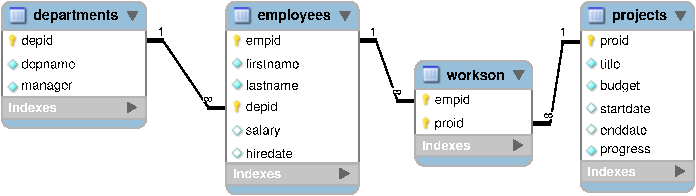
\includegraphics[scale=0.9]{../common/companyREL.pdf}
\end{minipage}
\end{frame}



\begin{frame}[t, fragile, shrink]
\frametitle{Πλήθος υπαλλήλων ανά έργο -- βήμα 1}
\begin{minipage}{\wE}
\vspace{-0.5cm}
\begin{block}{\small Σύζευξη πινάκων}
\[
  \begin{split}
      \varrho_{e} (employees) \bowtie_{e.empid=w.empid} \varrho_{w} (workson)  \\
                              \bowtie_{w.proid=p.proid} \varrho_{p} (projects)
  \end{split}
\]
\vspace{-0.5cm}
\pause
\en
\begin{SQL}
    FROM (employees e INNER JOIN workson w
                         ON e.empid = w.empid)
                      INNER JOIN projects p
                         ON w.proid = p.proid
\end{SQL}
\el
\end{block}
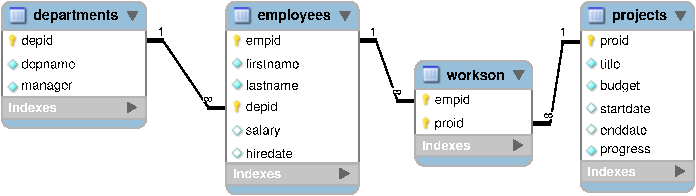
\includegraphics[scale=0.9]{../common/companyREL.pdf}
\end{minipage}
\end{frame}


\begin{frame}[t, fragile, shrink]
\frametitle{Πλήθος υπαλλήλων ανά έργο -- βήμα 2}
\begin{minipage}{\wE}
\vspace{-0.5cm}
\begin{block}{\small Περιορισμός εγγραφών {\en e.depid=4}}
Υπάρχει o περιορισμός που αφορά τους υπαλλήλους του τμήματος 4:
\[
\begin{split}
    \sigma_{e.depid=4}
    (                           \\
      \varrho_{e} (employees) \bowtie_{e.empid=w.empid} \varrho_{w} (workson)  \\
                              \bowtie_{w.proid=p.proid} \varrho_{p} (projects)
    )
\end{split}
\]
\vspace*{-1em}
\pause
\en
\begin{SQL}
    FROM (employees e INNER JOIN workson w
                         ON e.empid = w.empid)
                      INNER JOIN projects p
                         ON w.proid = p.proid
   WHERE e.depid = 4
\end{SQL}
\el
\end{block}
\end{minipage}
\end{frame}


\begin{frame}[t, fragile, shrink]
\frametitle{Πλήθος υπαλλήλων ανά έργο -- βήμα 3}
\begin{minipage}{\wE}
\vspace{-0.5cm}
\begin{block}{\small Ομαδοποίηση}
  «πλήθος των υπαλλήλων ανά έργο», δηλαδή {\crr ομαδοποίηση}:\\
\[
\begin{split}
  {}_{p.proid, p.title} \calg_{count(*)}
    (
      \sigma_{e.depid=4}
      (                           \\
        \varrho_{e} (employees) \bowtie_{e.empid=w.empid} \varrho_{w} (workson) \\
                                \bowtie_{w.proid=p.proid} \varrho_{p} (projects)
      )
    )
\end{split}
\]
\pause
\en
\begin{SQL}
    FROM (employees e INNER JOIN workson w
                         ON e.empid = w.empid)
                      INNER JOIN projects p
                         ON w.proid = p.proid
   WHERE e.depid = 4
GROUP BY p.proid, p.title
\end{SQL}
\el
\end{block}
\end{minipage}
\end{frame}


\begin{frame}[t, fragile, shrink]
\frametitle{Πλήθος υπαλλήλων ανά έργο -- βήμα 4}
\begin{minipage}{\wE}
\vspace{-0.5cm}
\begin{block}{\small Τελική διατύπωση}
\[
\begin{split}
      {}_{p.proid, p.title} \calg_{count(*)}
      (
        \sigma_{e.depid=2}
        (                           \\
          \varrho_{e} (employees) \bowtie_{e.empid=w.empid} \varrho_{w} (workson) \\
                                  \bowtie_{w.proid=p.proid} \varrho_{p} (projects)
        )
      )
\end{split}
\]
\pause
\en
\begin{SQL}
  SELECT p.proid, p.title, COUNT(*)
    FROM (employees e INNER JOIN workson  w
                         ON e.empid = w.empid)
                      INNER JOIN projects p
                         ON p.proid = w.proid
   WHERE e.depid = 4
GROUP BY p.proid, p.title;
\end{SQL}
\el
\end{block}
\end{minipage}
\end{frame}


